\documentclass[11pt]{article}

\usepackage{amsmath}
\usepackage{textcomp}
\usepackage[top=0.8in, bottom=0.8in, left=0.8in, right=0.8in]{geometry}
\usepackage{graphicx}
\graphicspath{ {img/} }
% Add other packages here %



% Put your group number and names in the author field %
\title{\bf Exercise 1.\\ Implementing a first Application in RePast: A Rabbits Grass Simulation.}
\author{Group 39: Hugo Bonnome, Pedro Amorim}

\begin{document}
\maketitle

\section{Implementation}

\subsection{Assumptions}
% Describe the assumptions of your world model and implementation (e.g. is the grass amount bounded in each cell) %
Our model made the following assumptions:
\begin{itemize}
\item The world is modelled as 2D grid where warping occurs at each edge, making
  it behave as a torus.
\item Agents can only give birth once per step.
\item If an agent tries to move to a cell that is currently occupied it will
  remain motionless during this time step instead.
\item The total amount of grass in a cell is bounded.
\item When a rabbit reaches a cell with grass, it will consume the total amount present in this cell.
\end{itemize}

\subsection{Implementation Remarks}
% Provide important details about your implementation, such as handling of boundary conditions %
\begin{itemize}
\item The torus behaviour of the grid is implemented with the help of modulus
  operations on the position coordinates.
\item At each time step of the simulation, each rabbit is checked to see if
  it has sufficient energy to reproduce. If that is the case then a new
  agent is added in a random position in the grid and the energy levels of
  the genitor rabbit are decreased by a preset amount.
\item At each time step each rabbit gets a random direction with the help of an
  enum encoding each cardinal direction (N,S,E,W). The potential new position of
  the rabbit is computed and then we check whether it would cause a collision.
  If a collision would indeed occur then the rabbit does not move during this
  time step.
\item At each time step a predefined amount of grass is added to the world and
  spread randomly. The amount of grass in a cell is implemented as an integer
  value. The bounding of the grass amount is simply implemented by taking the
  minimum of the maximum amount of grass in a cell and the updated value.
\end{itemize}
  
\section{Results}
% In this section, you study and describe how different variables (e.g. birth threshold, grass growth rate etc.) or combinations of variables influence the results. Different experiments with different settings are described below with your observations and analysis

\subsection{Experiment 1}

\subsubsection{Setting}
\begin{itemize}
\item Birth threshold: 80 units of energy
\item Grass growth rate: 10 units of grass per time step
\item Grid size: $20\times 20$ units
\item Initial number of agents: 5
\end{itemize}

\begin{figure}[h]
  \caption{Population plot of experiment 1}
  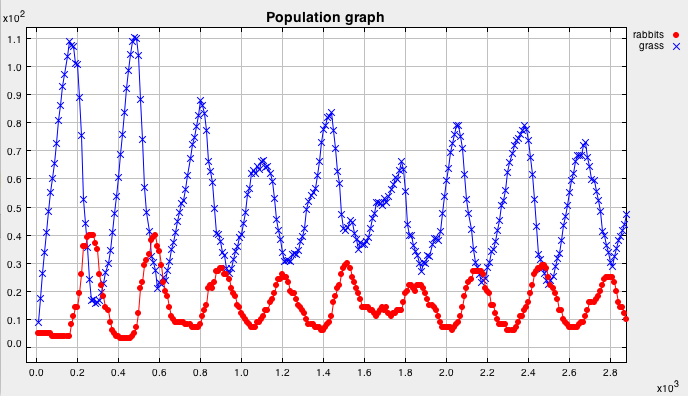
\includegraphics[width=0.75\textwidth]{experiment1}
  \centering
\end{figure}

\subsubsection{Observations}
% Elaborate on the observed results %
With these parameters the population follows the damped oscillations that are a
characteristic of prey predator models as described by Lotka-Volterra equations.

When the population of rabbits is low the grass has all the space to grow
freely. When the grass is abundant enough the rabbits have enough resources to
thrive and reproduce at a higher rate. This increase in rabbit population makes
the grass amounts decrease to a low until multiple rabbits start to starve. As
soon as the rabbit population drops down the grass can develop again and the
cycle restarts.

\subsection{Experiment 2}

\subsubsection{Setting}
Same as Experiment 1 but the birth threshold was changed to 60 units of energy.

\begin{figure}[h]
  \caption{Population plot of experiment 2}
  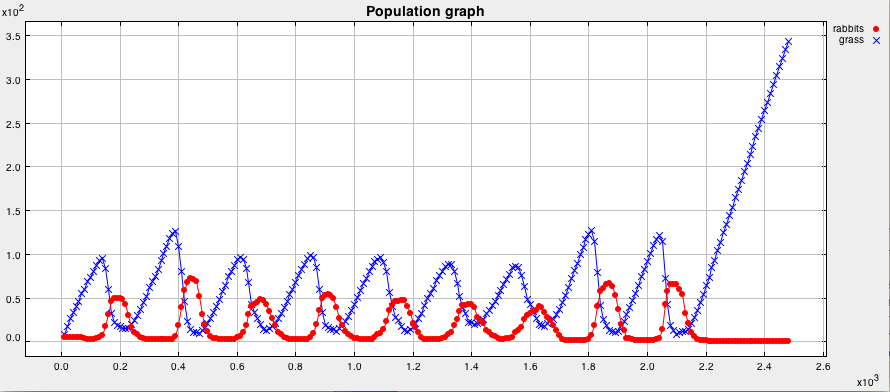
\includegraphics[width=0.75\textwidth]{experiment2}
  \centering
\end{figure}

\subsubsection{Observations}
% Elaborate on the observed results %
Since the birth threshold is lower, the population of rabbits increases much
more quickly. Overpopulation makes the competition for resources intense up
until the point where there is almost no grass left and the rabbits go extinct.

\subsection{Experiment 3}

\subsubsection{Setting}
Same as experiment 1 but the grass growth rate was doubled.

\begin{figure}[h]
  \caption{Population plot of experiment 3}
  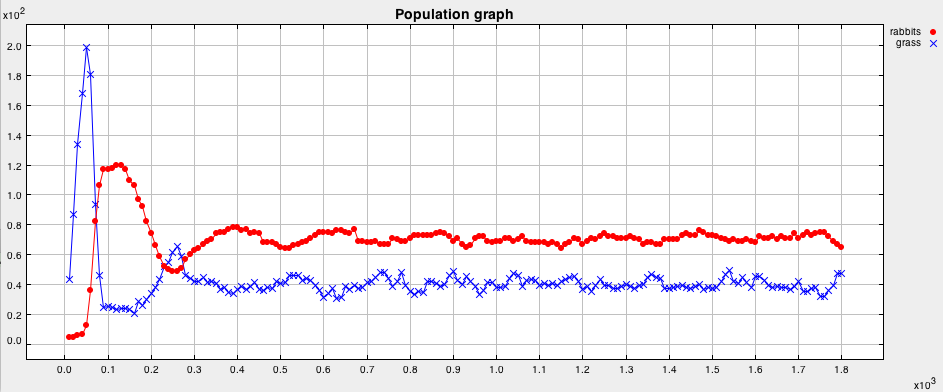
\includegraphics[width=0.75\textwidth]{experiment3}
  \centering
\end{figure}

\subsubsection{Observations}
% Elaborate on the observed results %
In this setting the grass is consumed at the same rate at which it grows. The
rabbits' deaths and births are also balanced. This results in population numbers
with almost no fluctuation.

\end{document}
